\hypertarget{functional-requirements}{%
\chapter{Functional Requirements}\label{functional-requirements}}

This chapters systematically lays out the functional requirements which
has to be implemented in the proof-of-concept application to satisfy the
1.7.2 scenario.

\hypertarget{functional-requirements-layers}{%
\section{Functional Requirements
Layers}\label{functional-requirements-layers}}

The become a full SSI agent, our proof-of-concept will have to implement
functionality across 4 distinct layers:

\begin{itemize}
\tightlist
\item
  \textbf{Layer 1:} DID
\item
  \textbf{Layer 2:} DIDComm
\item
  \textbf{Layer 3:} Verifiable Credentials
\item
  \textbf{Layer 4:} Application (Scenario)
\end{itemize}

The specific names I have used for the layers are based on my own
interpretation of the SSI stack. You will find that many different names
are used across the literature. Although the names of the layers are not
stable, there is a general agreement about the number of layers and
their scopes. Below is an image depicting an alternate view of the SSI
stack.

\begin{figure}
\centering
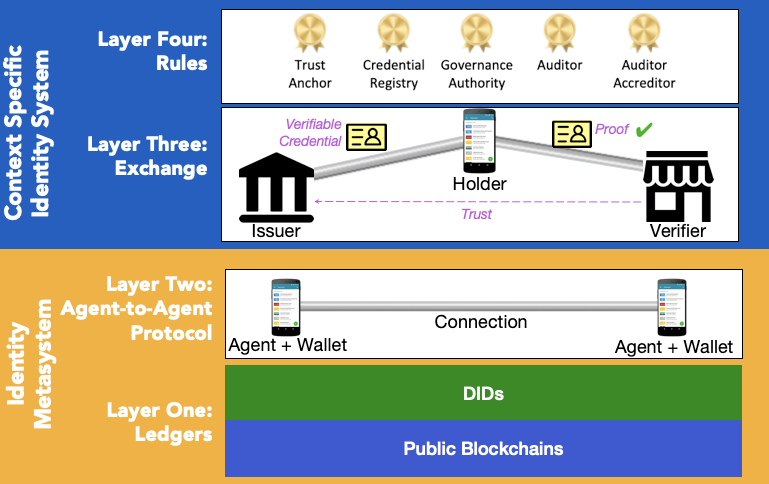
\includegraphics{Functional Requirements b66771c223f2424c9b1ba3285a2ba469/Untitled.png}
\caption{Untitled}
\end{figure}

Image: An alternative view of the \emph{Sovrin SSI stack -
\url{https://www.windley.com/archives/2020/03/the_sovrin_ssi_stack.shtml}}

\textbf{Sidenote on Sovrin:}

The image above refers the the Sovrin SSI stack. Sovrin is popular
alternative to Bitcoin and Ethereum as an SSI ledger. What
differentiates Sovrin from Ethereum and Bitcoin is that it is a ``public
permissioned'' blockchain, whereas Bitcoin and Ethereum is ``public
permissionless''.

\begin{figure}
\centering
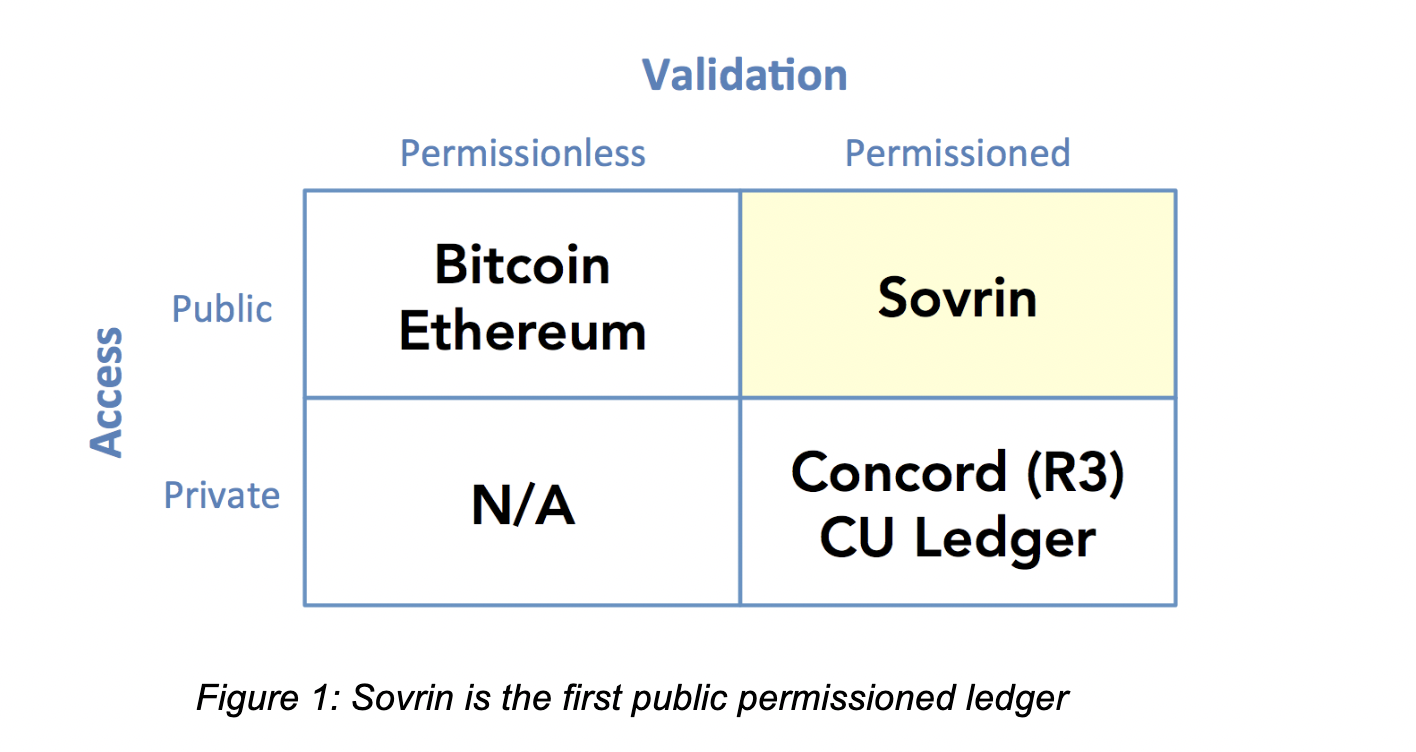
\includegraphics{Functional Requirements b66771c223f2424c9b1ba3285a2ba469/Untitled 1.png}
\caption{Untitled}
\end{figure}

\emph{Image from ``The Technical Foundations of Sovrin'' -
\url{https://www.evernym.com/wp-content/uploads/2017/07/The-Technical-Foundations-of-Sovrin.pdf}}

\hypertarget{bdd-style-requirements}{%
\section{BDD-style Requirements}\label{bdd-style-requirements}}

The rest of this chapter is heavily influenced by BDD (Behaviour Driven
Development). BDD is concerned how we should specify the behaviour of
the application we are developing. BDD states that we should write our
functional requirements describing behaviour in a human readable format.
In BDD all our requirements should be easily translatable to tests. BDD
is a tool for bridging the gap between technical engineers and
non-technical users of the software.

Here are some of quotes about the philosophy behind BDD:

\begin{itemize}
\tightlist
\item
  ``Test method names should be sentences''
\item
  ````Behaviour'' is a more useful word than ``test''''
\item
  ``Requirements are behaviour, too''
\item
  ``BDD provides a ``ubiquitous language'' for analysis''
\end{itemize}

\emph{See ``Introducing BDD'' by Dan North -
\url{http://dannorth.net/introducing-bdd/}}

\hypertarget{bdd-ubiquitous-language}{%
\subsection{BDD Ubiquitous Language}\label{bdd-ubiquitous-language}}

BDD ubiquitous language is the language we use when writing BDD-style
requirements.

\hypertarget{story-template}{%
\subsubsection{Story template}\label{story-template}}

A \textbf{story template} describes functionality we want to implement,
and is described like this:

\begin{quote}
\textbf{As a} {[}X{]} \textbf{I want} {[}Y{]} \textbf{so that} {[}Z{]}
\end{quote}

where Y is some feature, Z is the benefit or value of the feature, and X
is the person (or role) who will benefit. \textgreater{}

Example of valid \textbf{story-template:}

\begin{lstlisting}[language=bash]
**Title: Customer withdraws cash**

**As a** customer,
**I want** to withdraw cash from an ATM,
**so that** I don't have to wait in line at the bank.
\end{lstlisting}

\hypertarget{scenario-template}{%
\subsubsection{Scenario template}\label{scenario-template}}

The BDD ubiquitous language also provides a template for describing
different \textbf{scenarios} connected to the \textbf{story-template:}

\begin{lstlisting}[language=bash]
**Given** some initial context (the givens),  
**When** an event occurs,  
**Then** ensure some outcomes.
\end{lstlisting}

Here is an example of a valid \textbf{scenario:}

\begin{lstlisting}[language=bash]
**Scenario: Account is in credit**

**Given** the account is in credit
**And** the card is valid
**And** the dispenser contains cash
**When** the customer requests cash
**Then** ensure the account is debited
**And** ensure cash is dispensed
**And** ensure the card is returned
\end{lstlisting}

There could be multiple \textbf{scenarios} per feature:

\begin{lstlisting}[language=bash]
**Scenario: Account is overdrawn past the overdraft limit

Given** the account is overdrawn
**And** the card is valid
**When** the customer requests cash
**Then** ensure a rejection message is displayed
**And** ensure cash is not dispensed
**And** ensure the card is returned
\end{lstlisting}

\hypertarget{layer-1---did}{%
\section{Layer 1 - DID}\label{layer-1---did}}

Layer 1 is concerned with the creation of Self-sovereign agents, which
can be uniquely identified by a DID. As you will notice, each
sub-chapter from now on, will have a list of requirements written out as
user-stories.

\hypertarget{as-a-user-i-want-to-create-a-agent-inside-a-directory-on-my-machine}{%
\subsubsection{\texorpdfstring{\textbf{As a user I want to create a
agent inside a directory on my
machine}}{As a user I want to create a agent inside a directory on my machine}}\label{as-a-user-i-want-to-create-a-agent-inside-a-directory-on-my-machine}}

\begin{lstlisting}
**GIVEN** I am in an empty directory
**WHEN** I run *did init* (like *git init*)
**THEN** an agent should be created and stored in the sub-directory *.did/ (*like *.git/*)
    and ****all sub-sequent commands, when run from this directory, implicitly refers 
            to the agent stored in *.did*/ (like how all *git* commands implicitly refers
            to the git history stored in .git/).
\end{lstlisting}

Note: A directory initialised by \emph{did init} will from now on be
referred to as an agent-directory.

\hypertarget{as-a-user-i-want-to-view-an-agents-did}{%
\subsubsection{As a user I want to view an agent's
DID}\label{as-a-user-i-want-to-view-an-agents-did}}

\begin{lstlisting}
**GIVEN** I am in an agent-directory
**WHEN** I run *did init
    or* I run *did did self*
**THEN** the agent's DID should be written to *stdout*.
\end{lstlisting}

\hypertarget{as-a-user-i-want-to-view-an-agents-did-document}{%
\subsubsection{As a user I want to view an agent's DID
document}\label{as-a-user-i-want-to-view-an-agents-did-document}}

\begin{lstlisting}
**GIVEN** I am in an agent-directory
**WHEN** I run *did doc*
**THEN** the agent's DID-document should be written to *stdout* as prettified JSON.
\end{lstlisting}

\hypertarget{as-a-user-i-want-to-connect-a-name-to-a-did}{%
\subsubsection{As a user I want to connect a name to a
DID}\label{as-a-user-i-want-to-connect-a-name-to-a-did}}

\begin{lstlisting}
**GIVEN** I am in an agent-directory
    and I have a DID *did:key:z6Mkjid...*
**WHEN** I run *did connect doctor did:key:z6Mkjid...*
**THEN** the name *doctor* should be stored in my agent
    and I should be able to use *doctor* in other commands, instead of typing the 
        whole underlying DID.
    and the name *doctor* should be written to *stdout*, to enable chaining together 
        commands.
\end{lstlisting}

\hypertarget{as-a-user-i-want-to-refer-to-my-agents-did-by-using-the-name-self}{%
\subsubsection{\texorpdfstring{As a user I want to refer to my agent's
DID by using the name
\emph{self}}{As a user I want to refer to my agent's DID by using the name self}}\label{as-a-user-i-want-to-refer-to-my-agents-did-by-using-the-name-self}}

\begin{lstlisting}
**GIVEN** I am in an agent-directory
**WHEN** I run any command. Example: *did write self hello*
**THEN** the name *self* refers to my agents DID.
\end{lstlisting}

\hypertarget{as-a-user-i-want-to-view-all-my-dids}{%
\subsubsection{As a user I want to view all my
DID's}\label{as-a-user-i-want-to-view-all-my-dids}}

\begin{lstlisting}
**GIVEN** I am in an agent-directory
    and I there are some *names* stored in the agent
**WHEN** I run *did dids*
**THEN** a list of all the agent's stored names should be written to *stdout*.
\end{lstlisting}

\hypertarget{as-a-user-i-want-to-view-the-did-connected-to-a-name}{%
\subsubsection{As a user I want to view the DID connected to a
name}\label{as-a-user-i-want-to-view-the-did-connected-to-a-name}}

\begin{lstlisting}
**GIVEN** I am in an agent-directory
    and the agent has a name *police*
**WHEN** I run *did did police*
**THEN** the DID of *police* should be written to *stdout*.
\end{lstlisting}

\hypertarget{layer-2---didcomm}{%
\section{Layer 2 - DIDComm}\label{layer-2---didcomm}}

Layer 2 is concerned with \textbf{encrypting}, \textbf{sending},
\textbf{receiving} and \textbf{decrypting} DIDComm-messages between the
self-sovereign agents from Layer 1.

\hypertarget{as-a-user-i-want-to-write-a-dcem-from-one-agent-to-another}{%
\subsubsection{As a user I want to write a DCEM from one agent to
another}\label{as-a-user-i-want-to-write-a-dcem-from-one-agent-to-another}}

\begin{lstlisting}
**GIVEN** I have two agents on my machine
    **and** I am in one of the agent-directories
    **and** I have stored the DID of the other agent by the name *other*
**WHEN** I run *did write other hello*, with the contents "Hello"
**THEN** a DCEM should be written to *stdout*
    **and** the DCEM should be addressed to *other*.
\end{lstlisting}

For more info on DCEM - DIDComm Encrypted Message - see:
\href{https://identity.foundation/didcomm-messaging/spec/\%5C\%5C\#didcomm-encrypted-message}{https://identity.foundation/didcomm-messaging/spec/\textbackslash\#didcomm-encrypted-message}.

\hypertarget{as-a-user-i-want-to-read-the-contents-of-a-dcem-addressed-to-an-agent}{%
\subsubsection{As a user I want to read the contents of a DCEM addressed
to an
agent}\label{as-a-user-i-want-to-read-the-contents-of-a-dcem-addressed-to-an-agent}}

\begin{lstlisting}
**GIVEN** I am in an agent-directory
    **and** I receive a DCEM-file - *hello.dcem* - addressed to my agent
**WHEN** I run *did read $(cat hello.dcem)*
    **or** I run *cat hello.dcem | did read*
**THEN** the plaintext contents of the DCEM should be written to *stdout*.
\end{lstlisting}

\hypertarget{as-a-user-i-want-to-hold-a-dcem-inside-an-agent}{%
\subsubsection{As a user I want to hold a DCEM inside an
agent}\label{as-a-user-i-want-to-hold-a-dcem-inside-an-agent}}

\begin{lstlisting}
**GIVEN** I am in an agent-directory
    **and** I receive a DCEM-file - *hello.dcem* - addressed to my agent
**WHEN** I run *did hold \$(cat hello.dcem)}
    **or** I run *cat hello.dcem | did hold*
**THEN** the DCEM should be stored inside my agent with the id of the DCEM
    **and** the DCEM should be written to *stdout*.
\end{lstlisting}

If an existing DCEM has id=4, and a new DCEM also has id=4, then new
DCEM should overwrite the one already held by the agent (a message
received should be store idempotent).

\hypertarget{as-a-user-i-want-to-view-a-list-of-all-dcems-an-agent-is-holding}{%
\subsubsection{As a user I want to view a list of all DCEMs an agent is
holding}\label{as-a-user-i-want-to-view-a-list-of-all-dcems-an-agent-is-holding}}

\begin{lstlisting}
**Given** I am in an agent-directory
    **and** the agent is holding multiple DCEMs
**When** I run *did messages*
**Then** a list of all agent's DCEM-ids, should be written to *stdout*.
\end{lstlisting}

\hypertarget{as-a-user-i-want-to-view-a-single-dcem-an-agent-is-holding}{%
\subsubsection{As a user I want to view a single DCEM an agent is
holding}\label{as-a-user-i-want-to-view-a-single-dcem-an-agent-is-holding}}

\begin{lstlisting}
**GIVEN** I am in an agent-directory
    **and** there is a DCEM with id *7497036273686508746*, held by the agent
**WHEN** I run *did message 7497036273686508746*
**THEN** the DCEM should be written to *stdout.*
\end{lstlisting}

\hypertarget{layer-3---verifiable-credentials}{%
\section{Layer 3 - Verifiable
Credentials}\label{layer-3---verifiable-credentials}}

Layer 3 is concerned with the \textbf{issuing}, \textbf{holding},
\textbf{presenting} and \textbf{verifying} verifiable credentials and
passing these credentials over any transport which supports DIDComm from
Layer 2.

\hypertarget{as-an-issuer-i-want-to-issue-a-verifiable-credential-to-a-subject}{%
\subsubsection{As an issuer I want to issue a Verifiable Credential to a
subject}\label{as-an-issuer-i-want-to-issue-a-verifiable-credential-to-a-subject}}

\begin{lstlisting}
**GIVEN** I am in an agent-directory
    **and** the agent has connected a DID to the name *bob.*
**WHEN** I run *did issue Passport bob*
**THEN** a DCEM with a Verifiable Credential of type *Passport*, 
    **with** *vc.issuer.did* of *self*
    **with** the *vc.subject.did* of *bob* should be written to *stdout*.
\end{lstlisting}

\hypertarget{as-a-holder-i-want-to-present-a-verifiable-presentation-to-a-verifier}{%
\subsubsection{As a holder I want to present a Verifiable presentation
to a
verifier}\label{as-a-holder-i-want-to-present-a-verifiable-presentation-to-a-verifier}}

\begin{lstlisting}
**GIVEN** I am in an agent-directory
    **and** the agent has connected a DID to the name *police*
    **and** the agent is holding a Verifiable Credential as a DCEM with id 1234
**WHEN** I run *did message 1234 | did present police*
    **or** I run *did present Passport police $(did message 1234)*
**THEN** a DCEM with a Verifiable Presentation of type *Passport*, 
    **with** *vc.issuer.did* of *self*
    **with** *vp.holder.did* of *self*
    **with** the Verifiable Credential from *did message 1234*, 
    should be written to stout.
\end{lstlisting}

\hypertarget{as-a-verifier-i-want-to-verify-a-verifiable-presentation}{%
\subsubsection{As a verifier I want to verify a Verifiable
Presentation}\label{as-a-verifier-i-want-to-verify-a-verifiable-presentation}}

\begin{lstlisting}
**GIVEN** I am in an agent-directory
    **and** and the agent has connected a DID to the name *jonny*
    **and** and the agent has connected a DID to the name *police*
    **and** I have a file with a Verifiable Presentation of type *Passport*, stored as *passport.vp.dcem
WHEN* I run *cat passport.vp.dcem | did verify Passport police jonny*
    **or** I run *did verify Passport police jonny $(cat passport.vp.dcem)*
    **and** it succeeds
**Then** I can trust that the *vp.type* is *Passport*
    **and** that the *vp.vc.issuer.did* is *police*
    **and** that the *vp.vc.subject.did* is *jonny*
    **and** the file *passport.vp.dcem* will be written to *stdout*
\end{lstlisting}

\hypertarget{layer-4---application-scenario}{%
\section{Layer 4 - Application
(Scenario)}\label{layer-4---application-scenario}}

Layer 4 uses Layer 1, Layer 2 and Layer 3 to solve a real world problem.
The functional requirements specified here makes it possible to solve
the problem depicted in Scenario 1.7.2.

\hypertarget{as-a-citizen-i-want-to-publish-my-did-to-a-directory-other-citizens-can-access}{%
\subsubsection{As a citizen I want to publish my DID to a directory
other citizens can
access}\label{as-a-citizen-i-want-to-publish-my-did-to-a-directory-other-citizens-can-access}}

\begin{lstlisting}
**GIVEN** I am in my agent's directory
**WHEN** I run *did init > ../jonas.did*
    **or** I run *did did self > ../jonas.did*
**THEN** a file with the name *../jonas.did* should contain my DID.
\end{lstlisting}

\hypertarget{as-a-government-i-want-to-connect-to-my-citizens-agents}{%
\subsubsection{As a government I want to connect to my citizens'
agents}\label{as-a-government-i-want-to-connect-to-my-citizens-agents}}

\begin{lstlisting}
**GIVEN** I am in my agent's directory
    **and** my citizens each have their own agents
    **and** each citizen have published their DID as files *../snorre.did*, *abylay.did*, *jonas.did*
**WHEN** I run *cat jonas.did | did connect jonas*
    **and** I run *cat abylay.did | did connect abylay*
    **and** I run *cat snorre.did | did snorre snorre*
**THEN** I should be able to refer to my citizens by the names *jonas*, *abylay* and *snorre*, in other commands.
\end{lstlisting}

\hypertarget{as-a-citizen-i-want-to-connect-to-my-government-did}{%
\subsubsection{As a citizen I want to connect to my government
DID}\label{as-a-citizen-i-want-to-connect-to-my-government-did}}

\begin{lstlisting}
**GIVEN** I am in my agent's directory
    **and** my governemnt has a DID published in the file *../government.did*
**WHEN** I run *cat governemnt.did | did connect government*
**THEN** I should be able to refer to the name *government* in other commands.
\end{lstlisting}

\hypertarget{as-government-i-want-issue-passports-to-my-citizens-as-files}{%
\subsubsection{As government I want issue Passports to my citizens as
files}\label{as-government-i-want-issue-passports-to-my-citizens-as-files}}

\begin{lstlisting}
**GIVEN** I am in my agent's directory
    **and** my country has 3 citizens
    **and** I have connected to my citizens
**WHEN** I run *did issue Passport jonas > ../jonas.passport.vc.dcem*
    **and** I run *did issue Passport abylay > ../abylay.passport.vc.dcem*
    **and** I run *did issue Passport snorre > ../snorre.passport.vc.dcem*
**THEN** All my citizens should have access to a passport issued by me
    **and** one citizen should only be able to use the passport issued to him/her
    **and** one citizen should not be able to use the passport to issued others.
\end{lstlisting}

\hypertarget{as-a-citizen-i-want-to-hold-passports-issued-to-me}{%
\subsubsection{As a citizen I want to hold Passports issued to
me}\label{as-a-citizen-i-want-to-hold-passports-issued-to-me}}

\begin{lstlisting}
**GIVEN** I am in my agent's directory
    **and** my government has issued a Passport to in a file *../jonas.passport.vc.dcem*
**WHEN** I run *cat ../jonas.passport.vc.dcem | did hold*
**THEN** the Passport is stored in my agent as a DCEM.
\end{lstlisting}

\hypertarget{as-a-citizen-i-want-to-view-my-passport-in-plaintext}{%
\subsubsection{As a citizen I want to view my Passport in
plaintext}\label{as-a-citizen-i-want-to-view-my-passport-in-plaintext}}

\begin{lstlisting}
**GIVEN** I am in my agent's directory
    **and** I have am holding a Passport as a DCEM with id 1234
**WHEN** I run *did message 1234 | did read*
**THEN** my Passport should be written to *stdout* in plaintext.
\end{lstlisting}

\hypertarget{as-a-citizen-i-want-to-present-my-passport-to-the-police}{%
\subsubsection{As a citizen I want to present my Passport to the
Police}\label{as-a-citizen-i-want-to-present-my-passport-to-the-police}}

\begin{lstlisting}
**GIVEN** I am in my agent's directory
    **and** I have am holding a Passport as a DCEM with id 1234
    **and** I have connected a DID to the name *police*
**WHEN** I run *did message 1234 | did present police > ../jonas.passport.vp.dcem*
**THEN** my Passport should be stored in a file as a Verifiable Presentation
    **and** it should only be able to be viewed and verified by *police*
    **and** nobody else.
\end{lstlisting}

\hypertarget{as-the-police-i-want-to-verify-a-passport-from-a-citizen-i-am-controlling}{%
\subsubsection{As the Police I want to verify a Passport from a citizen
I am
controlling}\label{as-the-police-i-want-to-verify-a-passport-from-a-citizen-i-am-controlling}}

\begin{lstlisting}
**GIVEN** I am in my agent's directory
    **and** I have approached a citizen which has a agent
    **and** the citizens DID is stored in my agent with name *jonas*
    **and** the government's DID is stored in my agent with name *government*
    **and** the citizen presents his passport to me as the file 
        *../jonas.passport.vp.dcem*
**WHEN** I run *cat ../jonas.passport.vp.dcem* | did verify Passport government *jonas*
**THEN** I can be sure that Verifiable Presentation is of type *Passport*
    **and** and is issued by the *government*
    **and** and has a subject of *jonas.*
\end{lstlisting}
